%%%%%%%%%%%%%%%%%%%%%%%%%%%%%%%%%%%%%%%%%
%  My documentation report
%  Objetive: Explain what I did and how, so someone can continue with the investigation
%
% Important note:
% Chapter heading images should have a 2:1 width:height ratio,
% e.g. 920px width and 460px height.
%
%%%%%%%%%%%%%%%%%%%%%%%%%%%%%%%%%%%%%%%%%

%----------------------------------------------------------------------------------------
%	PACKAGES AND OTHER DOCUMENT CONFIGURATIONS
%----------------------------------------------------------------------------------------

\documentclass[11pt,fleqn]{book} % Default font size and left-justified equations

\usepackage[top=3cm,bottom=3cm,left=3.2cm,right=3.2cm,headsep=10pt,letterpaper]{geometry} % Page margins

\usepackage{xcolor} % Required for specifying colors by name
\definecolor{darkgreen}{RGB}{0, 153, 0} % Define the orange color used for highlighting throughout the book

% Font Settings
\usepackage{avant} % Use the Avantgarde font for headings
%\usepackage{times} % Use the Times font for headings
\usepackage{mathptmx} % Use the Adobe Times Roman as the default text font together with math symbols from the Sym­bol, Chancery and Com­puter Modern fonts

\usepackage{microtype} % Slightly tweak font spacing for aesthetics
\usepackage[utf8]{inputenc} % Required for including letters with accents
\usepackage[T1]{fontenc} % Use 8-bit encoding that has 256 glyphs

% Bibliography
\usepackage[style=alphabetic,sorting=nyt,sortcites=true,autopunct=true,babel=hyphen,hyperref=true,abbreviate=false,backref=true,backend=biber]{biblatex}
\addbibresource{bibliography.bib} % BibTeX bibliography file
\defbibheading{bibempty}{}

%----------------------------------------------------------------------------------------
%	VARIOUS REQUIRED PACKAGES
%----------------------------------------------------------------------------------------

\usepackage{titlesec} % Allows customization of titles

\usepackage{graphicx} % Required for including pictures
\graphicspath{{Pictures/}} % Specifies the directory where pictures are stored

\usepackage{lipsum} % Inserts dummy text

\usepackage{tikz} % Required for drawing custom shapes

\usepackage[english]{babel} % English language/hyphenation

\usepackage{enumitem} % Customize lists
\setlist{nolistsep} % Reduce spacing between bullet points and numbered lists

\usepackage{booktabs} % Required for nicer horizontal rules in tables

\usepackage{eso-pic} % Required for specifying an image background in the title page

%----------------------------------------------------------------------------------------
%	MAIN TABLE OF CONTENTS
%----------------------------------------------------------------------------------------

\usepackage{titletoc} % Required for manipulating the table of contents

\contentsmargin{0cm} % Removes the default margin
% Chapter text styling
\titlecontents{chapter}[1.25cm] % Indentation
{\addvspace{15pt}\large\sffamily\bfseries} % Spacing and font options for chapters
{\color{darkgreen!60}\contentslabel[\Large\thecontentslabel]{1.25cm}\color{darkgreen}} % Chapter number
{}  
{\color{darkgreen!60}\normalsize\sffamily\bfseries\;\titlerule*[.5pc]{.}\;\thecontentspage} % Page number
% Section text styling
\titlecontents{section}[1.25cm] % Indentation
{\addvspace{5pt}\sffamily\bfseries} % Spacing and font options for sections
{\contentslabel[\thecontentslabel]{1.25cm}} % Section number
{}
{\sffamily\hfill\color{black}\thecontentspage} % Page number
[]
% Subsection text styling
\titlecontents{subsection}[1.25cm] % Indentation
{\addvspace{1pt}\sffamily\small} % Spacing and font options for subsections
{\contentslabel[\thecontentslabel]{1.25cm}} % Subsection number
{}
{\sffamily\;\titlerule*[.5pc]{.}\;\thecontentspage} % Page number
[] 

%----------------------------------------------------------------------------------------
%	MINI TABLE OF CONTENTS IN CHAPTER HEADS
%----------------------------------------------------------------------------------------

% Section text styling
\titlecontents{lsection}[0em] % Indendating
{\footnotesize\sffamily} % Font settings
{}
{}
{}

% Subsection text styling
\titlecontents{lsubsection}[.5em] % Indentation
{\normalfont\footnotesize\sffamily} % Font settings
{}
{}
{}
 
%----------------------------------------------------------------------------------------
%	PAGE HEADERS
%----------------------------------------------------------------------------------------

\usepackage{fancyhdr} % Required for header and footer configuration

\pagestyle{fancy}
\renewcommand{\chaptermark}[1]{\markboth{\sffamily\normalsize\bfseries\chaptername\ \thechapter.\ #1}{}} % Chapter text font settings
\renewcommand{\sectionmark}[1]{\markright{\sffamily\normalsize\thesection\hspace{5pt}#1}{}} % Section text font settings
\fancyhf{} \fancyhead[LE,RO]{\sffamily\normalsize\thepage} % Font setting for the page number in the header
\fancyhead[LO]{\rightmark} % Print the nearest section name on the left side of odd pages
\fancyhead[RE]{\leftmark} % Print the current chapter name on the right side of even pages
\renewcommand{\headrulewidth}{0.5pt} % Width of the rule under the header
\addtolength{\headheight}{2.5pt} % Increase the spacing around the header slightly
\renewcommand{\footrulewidth}{0pt} % Removes the rule in the footer
\fancypagestyle{plain}{\fancyhead{}\renewcommand{\headrulewidth}{0pt}} % Style for when a plain pagestyle is specified

% Removes the header from odd empty pages at the end of chapters
\makeatletter
\renewcommand{\cleardoublepage}{
\clearpage\ifodd\c@page\else
\hbox{}
\vspace*{\fill}
\thispagestyle{empty}
\newpage
\fi}

%----------------------------------------------------------------------------------------
%	THEOREM STYLES
%----------------------------------------------------------------------------------------

\usepackage{amsmath,amsfonts,amssymb,amsthm} % For math equations, theorems, symbols, etc

\newcommand{\intoo}[2]{\mathopen{]}#1\,;#2\mathclose{[}}
\newcommand{\ud}{\mathop{\mathrm{{}d}}\mathopen{}}
\newcommand{\intff}[2]{\mathopen{[}#1\,;#2\mathclose{]}}
\newtheorem{notation}{Notation}[chapter]

%%%%%%%%%%%%%%%%%%%%%%%%%%%%%%%%%%%%%%%%%%%%%%%%%%%%%%%%%%%%%%%%%%%%%%%%%%%
%%%%%%%%%%%%%%%%%%%% dedicated to boxed/framed environements %%%%%%%%%%%%%%
%%%%%%%%%%%%%%%%%%%%%%%%%%%%%%%%%%%%%%%%%%%%%%%%%%%%%%%%%%%%%%%%%%%%%%%%%%%
\newtheoremstyle{ocrenumbox}% % Theorem style name
{0pt}% Space above
{0pt}% Space below
{\normalfont}% % Body font
{}% Indent amount
{\small\bf\sffamily\color{darkgreen}}% % Theorem head font
{\;}% Punctuation after theorem head
{0.25em}% Space after theorem head
{\small\sffamily\color{darkgreen}\thmname{#1}\nobreakspace\thmnumber{\@ifnotempty{#1}{}\@upn{#2}}% Theorem text (e.g. Theorem 2.1)
\thmnote{\nobreakspace\the\thm@notefont\sffamily\bfseries\color{black}---\nobreakspace#3.}} % Optional theorem note
\renewcommand{\qedsymbol}{$\blacksquare$}% Optional qed square

\newtheoremstyle{blacknumex}% Theorem style name
{5pt}% Space above
{5pt}% Space below
{\normalfont}% Body font
{} % Indent amount
{\small\bf\sffamily}% Theorem head font
{\;}% Punctuation after theorem head
{0.25em}% Space after theorem head
{\small\sffamily{\tiny\ensuremath{\blacksquare}}\nobreakspace\thmname{#1}\nobreakspace\thmnumber{\@ifnotempty{#1}{}\@upn{#2}}% Theorem text (e.g. Theorem 2.1)
\thmnote{\nobreakspace\the\thm@notefont\sffamily\bfseries---\nobreakspace#3.}}% Optional theorem note

\newtheoremstyle{blacknumbox} % Theorem style name
{0pt}% Space above
{0pt}% Space below
{\normalfont}% Body font
{}% Indent amount
{\small\bf\sffamily}% Theorem head font
{\;}% Punctuation after theorem head
{0.25em}% Space after theorem head
{\small\sffamily\thmname{#1}\nobreakspace\thmnumber{\@ifnotempty{#1}{}\@upn{#2}}% Theorem text (e.g. Theorem 2.1)
\thmnote{\nobreakspace\the\thm@notefont\sffamily\bfseries---\nobreakspace#3.}}% Optional theorem note

%%%%%%%%%%%%%%%%%%%%%%%%%%%%%%%%%%%%%%%%%%%%%%%%%%%%%%%%%%%%%%%%%%%%%%%%%%%
%%%%%%%%%%%%% dedicated to non-boxed/non-framed environements %%%%%%%%%%%%%
%%%%%%%%%%%%%%%%%%%%%%%%%%%%%%%%%%%%%%%%%%%%%%%%%%%%%%%%%%%%%%%%%%%%%%%%%%%
\newtheoremstyle{ocrenum}% % Theorem style name
{5pt}% Space above
{5pt}% Space below
{\normalfont}% % Body font
{}% Indent amount
{\small\bf\sffamily\color{darkgreen}}% % Theorem head font
{\;}% Punctuation after theorem head
{0.25em}% Space after theorem head
{\small\sffamily\color{darkgreen}\thmname{#1}\nobreakspace\thmnumber{\@ifnotempty{#1}{}\@upn{#2}}% Theorem text (e.g. Theorem 2.1)
\thmnote{\nobreakspace\the\thm@notefont\sffamily\bfseries\color{black}---\nobreakspace#3.}} % Optional theorem note
\renewcommand{\qedsymbol}{$\blacksquare$}% Optional qed square
\makeatother

% Defines the theorem text style for each type of theorem to one of the three styles above
\newcounter{dummy} 
\numberwithin{dummy}{section}
\theoremstyle{ocrenumbox}
\newtheorem{theoremeT}[dummy]{Theorem}
\newtheorem{problem}{Problem}[chapter]
\newtheorem{exerciseT}{Exercise}[chapter]
\theoremstyle{blacknumex}
\newtheorem{exampleT}{Example}[chapter]
\theoremstyle{blacknumbox}
\newtheorem{vocabulary}{Vocabulary}[chapter]
\newtheorem{definitionT}{Definition}[section]
\newtheorem{corollaryT}[dummy]{Corollary}
\theoremstyle{ocrenum}
\newtheorem{proposition}[dummy]{Proposition}

%----------------------------------------------------------------------------------------
%	DEFINITION OF COLORED BOXES
%----------------------------------------------------------------------------------------

\RequirePackage[framemethod=default]{mdframed} % Required for creating the theorem, definition, exercise and corollary boxes

% Theorem box
\newmdenv[skipabove=7pt,
skipbelow=7pt,
backgroundcolor=black!5,
linecolor=darkgreen,
innerleftmargin=5pt,
innerrightmargin=5pt,
innertopmargin=5pt,
leftmargin=0cm,
rightmargin=0cm,
innerbottommargin=5pt]{tBox}

% Exercise box	  
\newmdenv[skipabove=7pt,
skipbelow=7pt,
rightline=false,
leftline=true,
topline=false,
bottomline=false,
backgroundcolor=darkgreen!10,
linecolor=darkgreen,
innerleftmargin=5pt,
innerrightmargin=5pt,
innertopmargin=5pt,
innerbottommargin=5pt,
leftmargin=0cm,
rightmargin=0cm,
linewidth=4pt]{eBox}	

% Definition box
\newmdenv[skipabove=7pt,
skipbelow=7pt,
rightline=false,
leftline=true,
topline=false,
bottomline=false,
linecolor=darkgreen,
innerleftmargin=5pt,
innerrightmargin=5pt,
innertopmargin=0pt,
leftmargin=0cm,
rightmargin=0cm,
linewidth=4pt,
innerbottommargin=0pt]{dBox}	

% Corollary box
\newmdenv[skipabove=7pt,
skipbelow=7pt,
rightline=false,
leftline=true,
topline=false,
bottomline=false,
linecolor=gray,
backgroundcolor=black!5,
innerleftmargin=5pt,
innerrightmargin=5pt,
innertopmargin=5pt,
leftmargin=0cm,
rightmargin=0cm,
linewidth=4pt,
innerbottommargin=5pt]{cBox}

% Creates an environment for each type of theorem and assigns it a theorem text style from the "Theorem Styles" section above and a colored box from above
\newenvironment{theorem}{\begin{tBox}\begin{theoremeT}}{\end{theoremeT}\end{tBox}}
\newenvironment{exercise}{\begin{eBox}\begin{exerciseT}}{\hfill{\color{darkgreen}\tiny\ensuremath{\blacksquare}}\end{exerciseT}\end{eBox}}				  
\newenvironment{definition}{\begin{dBox}\begin{definitionT}}{\end{definitionT}\end{dBox}}	
\newenvironment{example}{\begin{exampleT}}{\hfill{\tiny\ensuremath{\blacksquare}}\end{exampleT}}		
\newenvironment{corollary}{\begin{cBox}\begin{corollaryT}}{\end{corollaryT}\end{cBox}}	

%----------------------------------------------------------------------------------------
%	REMARK ENVIRONMENT
%----------------------------------------------------------------------------------------

\newenvironment{remark}{\par\vspace{10pt}\small % Vertical white space above the remark and smaller font size
\begin{list}{}{
\leftmargin=35pt % Indentation on the left
\rightmargin=25pt}\item\ignorespaces % Indentation on the right
\makebox[-2.5pt]{\begin{tikzpicture}[overlay]
\node[draw=darkgreen!60,line width=1pt,circle,fill=darkgreen!25,font=\sffamily\bfseries,inner sep=2pt,outer sep=0pt] at (-15pt,0pt){\textcolor{darkgreen}{R}};\end{tikzpicture}} % Orange R in a circle
\advance\baselineskip -1pt}{\end{list}\vskip5pt} % Tighter line spacing and white space after remark

%----------------------------------------------------------------------------------------
%	SECTION NUMBERING IN THE MARGIN
%----------------------------------------------------------------------------------------

\makeatletter
\renewcommand{\@seccntformat}[1]{\llap{\textcolor{darkgreen}{\csname the#1\endcsname}\hspace{1em}}}                    
\renewcommand{\section}{\@startsection{section}{1}{\z@}
{-4ex \@plus -1ex \@minus -.4ex}
{1ex \@plus.2ex }
{\normalfont\large\sffamily\bfseries}}
\renewcommand{\subsection}{\@startsection {subsection}{2}{\z@}
{-3ex \@plus -0.1ex \@minus -.4ex}
{0.5ex \@plus.2ex }
{\normalfont\sffamily\bfseries}}
\renewcommand{\subsubsection}{\@startsection {subsubsection}{3}{\z@}
{-2ex \@plus -0.1ex \@minus -.2ex}
{.2ex \@plus.2ex }
{\normalfont\small\sffamily\bfseries}}                        
\renewcommand\paragraph{\@startsection{paragraph}{4}{\z@}
{-2ex \@plus-.2ex \@minus .2ex}
{.1ex}
{\normalfont\small\sffamily\bfseries}}

%----------------------------------------------------------------------------------------
%	HYPERLINKS IN THE DOCUMENTS
%----------------------------------------------------------------------------------------

% For an unclear reason, the package should be loaded now and not later
\usepackage{hyperref}
\hypersetup{hidelinks,backref=true,pagebackref=true,hyperindex=true,colorlinks=false,breaklinks=true,urlcolor= darkgreen,bookmarks=true,bookmarksopen=false,pdftitle={Title},pdfauthor={Author}}

%----------------------------------------------------------------------------------------
%	CHAPTER HEADINGS
%----------------------------------------------------------------------------------------

% The set-up below should be (sadly) manually adapted to the overall margin page septup controlled by the geometry package loaded in the main.tex document. It is possible to implement below the dimensions used in the goemetry package (top,bottom,left,right)... TO BE DONE

\newcommand{\thechapterimage}{}
\newcommand{\chapterimage}[1]{\renewcommand{\thechapterimage}{#1}}

% Numbered chapters with mini tableofcontents
\def\thechapter{\arabic{chapter}}
\def\@makechapterhead#1{
\thispagestyle{empty}
{\centering \normalfont\sffamily
\ifnum \c@secnumdepth >\m@ne
\if@mainmatter
\startcontents
\begin{tikzpicture}[remember picture,overlay]
\node at (current page.north west)
{\begin{tikzpicture}[remember picture,overlay]
\node[anchor=north west,inner sep=0pt] at (0,0) {\includegraphics[width=\paperwidth]{\thechapterimage}};
%%%%%%%%%%%%%%%%%%%%%%%%%%%%%%%%%%%%%%%%%%%%%%%%%%%%%%%%%%%%%%%%%%%%%%%%%%%%%%%%%%%%%
% Commenting the 3 lines below removes the small contents box in the chapter heading
%\fill[color=darkgreen!10!white,opacity=.6] (1cm,0) rectangle (8cm,-7cm);
%\node[anchor=north west] at (1.1cm,.35cm) {\parbox[t][8cm][t]{6.5cm}{\huge\bfseries\flushleft \printcontents{l}{1}{\setcounter{tocdepth}{2}}}};
\draw[anchor=west] (5cm,-9cm) node [rounded corners=20pt,fill=darkgreen!10!white,text opacity=1,draw=darkgreen,draw opacity=1,line width=1.5pt,fill opacity=.6,inner sep=12pt]{\huge\sffamily\bfseries\textcolor{black}{\thechapter. #1\strut\makebox[22cm]{}}};
%%%%%%%%%%%%%%%%%%%%%%%%%%%%%%%%%%%%%%%%%%%%%%%%%%%%%%%%%%%%%%%%%%%%%%%%%%%%%%%%%%%%%
\end{tikzpicture}};
\end{tikzpicture}}
\par\vspace*{230\p@}
\fi
\fi}

% Unnumbered chapters without mini tableofcontents (could be added though) 
\def\@makeschapterhead#1{
\thispagestyle{empty}
{\centering \normalfont\sffamily
\ifnum \c@secnumdepth >\m@ne
\if@mainmatter
\begin{tikzpicture}[remember picture,overlay]
\node at (current page.north west)
{\begin{tikzpicture}[remember picture,overlay]
\node[anchor=north west,inner sep=0pt] at (0,0) {\includegraphics[width=\paperwidth]{\thechapterimage}};
\draw[anchor=west] (5cm,-9cm) node [rounded corners=20pt,fill=darkgreen!10!white,fill opacity=.6,inner sep=12pt,text opacity=1,draw=darkgreen,draw opacity=1,line width=1.5pt]{\huge\sffamily\bfseries\textcolor{black}{#1\strut\makebox[22cm]{}}};
\end{tikzpicture}};
\end{tikzpicture}}
\par\vspace*{230\p@}
\fi
\fi
}
\makeatother % Insert the commands.tex file which contains the majority of the structure behind the template

\begin{document}
	
	%----------------------------------------------------------------------------------------
	%	TITLE PAGE
	%----------------------------------------------------------------------------------------
	
	\begingroup
	\thispagestyle{empty}
	\AddToShipoutPicture*{\put(0,0){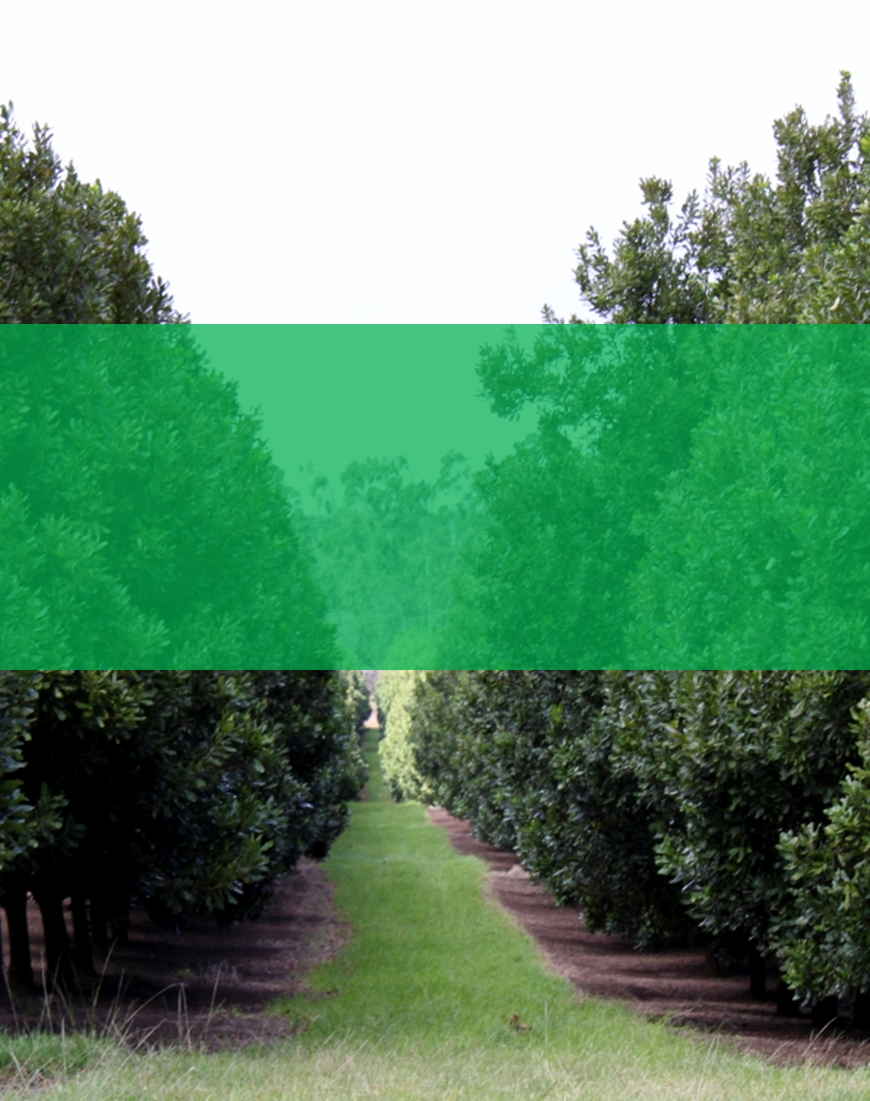
\includegraphics[scale=1]{frontcover}}} % Image background
	\centering
	\vspace*{5cm}
	\par\normalfont\fontsize{35}{35}\sffamily\selectfont
	\textbf{Harvest}\\
	{\LARGE Software Architectural Requirements and Design}\par % Book title
	\vspace*{0.5cm}
	{\Huge HTTP\_418}\par
	\centering
	\vspace*{0.5cm}
	\begin{itemize}[label={}, noitemsep]	
		\Large
		\item \begin{center} Christiaan Saaiman, 12059138 \end{center}
		\item \begin{center} Michael Loosen, 14017254 \end{center}
		\item \begin{center} Elizabeth Bode, 14310156 \end{center}
		\item \begin{center} LC Meyers, 14024633 \end{center}	
	\end{itemize}
	\endgroup
	
	%----------------------------------------------------------------------------------------
	%	TABLE OF CONTENTS
	%----------------------------------------------------------------------------------------
	
	\chapterimage{orchard.png} % Table of contents heading image
	
	\pagestyle{empty} % No headers
	
	\tableofcontents % Print the table of contents itself
	
	%\cleardoublepage % Forces the first chapter to start on an odd page so it's on the right
	
	\pagestyle{fancy} % Print headers again
	
	%----------------------------------------------------------------------------------------
	%	CHAPTER 1
	%----------------------------------------------------------------------------------------
	
	\chapterimage{mangoes.png} % Chapter heading image
	
	\chapter{Vision}
		The client, Subtrop, has requested that we implement a system to keep track of the crop yields of farms registered with them. The scope of the system entails managing the administration involved in the tracking of yields and the performance of the farm workers. Currently, this is done by manual tracking on a paper-based system. The system is required to keep track of all yield data and the associated farm’s metadata.\newline
		The current paper-based system consists of various farmers, their farms, the foreman they have appointed, their workers that work under the foreman and the different Subtrop crop type associations. Farms are divided into orchard blocks with each block having one crop type associated with it. Workers are paid according to their performance and, thus, this data has to be recorded. These two factors provide the potential for statistical data reports, which could aid farmers in strategic decision-making.\newline
		The most fundamental requirements that the client would like the system to fulfil are:
	\begin{itemize}
	\itemKeeping track of yield data in order to see which orchards are successful
	\itemKeeping track of worker performance in order to ensure that they are working to their full potential
	\end{itemize}

	
	
	%----------------------------------------------------------------------------------------
	%	CHAPTER 2
	%----------------------------------------------------------------------------------------
	\chapterimage{macadamias.png}
	
	\chapter{Background}
	\begin{itemize}
		\item Limitations of current system\newline\newline
		The current system being used by the client involves manually tracking worker performance with the use of a clipboard, with a list of all the workers names, and a pen.  The farmers have to manually record every yield that each worker collects in order to track their performance to determine their wages. The current system is inefficient due to the tedious nature of it. This tediousness reduces the foreman’s productivity as time is wasted unnecessarily searching for workers in the list and keeping track of all the lists chronologically. As the foreman is in charge of the workers, the workers have to wait until the yield they collected has been recorded which in turn also reduces their productivity.\newline
		
		\item High theft issue\newline\newline
		Farmers in the subtropical growers industry are continuously burdened by theft of their products by their own employees. This results in decreased revenue, increased costs, reduced productivity and a decrease in employer-employee trust, which creates the potential for a poor working environment. All of which necessitates the development of a new system that seeks to reduce the probability of crime by implementing monitoring on the foreman’s devices.\newline
		
		\item Need for statistical data\newline\newline
		The potential for generating statistical data that could aid farmers in future decisions from the manual data they collect is immense. The current paper-based storage of data prevents the generation of statistical reports due to the immense workload and time it requires. There is a huge need for reports indicating the highest producing orchard blocks, appropriate allocation of orchard block conditions to crop types and expected revenue. All of which could assist the farmers in future strategic planning.
	\end{itemize}
	%----------------------------------------------------------------------------------------
	%	CHAPTER 3
	%----------------------------------------------------------------------------------------
	
	\chapterimage{avocados.png}
	\chapter{Architecture Requirements}
	
	\section{Architectural Scope}
	\section{Access Channel Requirements}
	\subsection{Human Access Channels}
	\subsection{System Access Channels}
	
	\section{Quality Requirements}
	\subsection{Performance}
	\subsection{Reliability}
	\subsection{Scalability}
	\subsection{Security}
	\subsection{Flexibility}
	\subsection{Maintainability}
	\subsection{Auditability/Monitorability}
	\subsection{Integrability}
	\subsection{Cost}
	\subsection{Usability}
	
	\section{Integration Requirements}
	
	\section{Architecture Constraints}
	\subsection{Architectural Patterns}
	
	%----------------------------------------------------------------------------------------
	%	CHAPTER 4
	%----------------------------------------------------------------------------------------
	
	\chapterimage{litchis.png} % Chapter heading image
	
	\chapter{Architectural Tactics or Strategies}
	
	\section{Software Engineering Context : Architectural Tactics}
	\section{Performance Tactics}
	\subsection{Three Groups of Performance Tactics}
	\subsection{System Context}
	\section{Reliability Tactics}
	\subsection{System Context}
	\section{Scalability Tactics}
	\subsection{System Context}
	\section{Security Tactics}
	Security refers to the protection of information systems from unauthorized disruption that could potentially result in the corruption of information. It is achieved by enforcing access controls on individuals, according to a user hierarchy, to ensure only permitted users have access to the necessary information.
	\subsection{System Context}
	\begin{itemize}
		\item Resistance to SQL injections\newline\newline
		SQL injections are dependent on data type awareness in order to be successful. To prevent this, the data being transferred will be encrypted to hide its data type so only the system can understand it. All authentication data will be stored in an encrypted form and never in plain-text.\newline
		
		\item Enforce access rights according to user hierarchy \newline\newline
		The different users of the system, such as the farmer and the foremen, will have different access rights accordingly. The farmer will be a super user and will, thus, have access to all functionality that the system offers. The foremen will be general users and have restricted access to administration functionalities. This will simply be enforced by enabling and disabling certain functionalities according to user logins.\newline
		
		\item Password encryption\newline\newline
		Upon registration of a user account, the user’s password will be stored in the database after it has been automatically hashed. When the user logs in, the hashed password will be retrieved and converted to plain-text to perform authentication. No passwords will be stored in the database in plain-text format.\newline
		
		\item Enforce database authentication\newline\newline
		Access to database queries will be limited according to the aforementioned user hierarchy. The farmer will have direct access to view and modify the database whereas the foremen will only be able to make additions to the database regarding worker performance.			
	\end{itemize}
	\section{Flexibility Tactics}
	\subsection{System Context}
	\section{Maintainability Tactics}
	Maintainability refers to modifying the existing system to make improvements or fix bugs without jeopardizing the data integrity and functionality. The need for maintainability is usually based on the following factors: changes in the software environment, new user requirements, bug and error fixes and the requirement of preventative measures for future problems.
	\subsection{System Context}
	\begin{itemize}
		\item Enforce code documentation\newline\newline
		JSDoc will be enforced as the documentation framework as its sole purpose is to generate documentation for JavaScript, the language which the whole system will be based on. This will ensure that other developers will always be able to understand what is going on in the code.\newline
		
		\item Setup coding standards and conventions\newline\newline
		The CSS3 files should be sorted alphabetically to aid in navigation and understanding for other developers. Other good practices such as naming conventions for variables, functions and classes should be specified to ensure consistency and readability throughout.\newline
		
		\item Enforce modularization of system components\newline\newline
		The system should separate concerns by dividing the system components into distinct and independent modules to improve maintainability. This will be enforced with the use of various frameworks such as Node.js, Express,js, Sails,js and Angular.js, which require separation of concerns as they are MVC-oriented.
		
	\end{itemize}
	\section{Auditability Tactics}
	\subsection{System Context}
	\section{Integrability and Extensibility Tactics}
	\subsection{System Context}
	\section{Cost Tactics}
	Costs refer to all the funding required in order for the system to function fully. These costs include development costs, operational costs and maintenance costs.
	\subsection{System Context}
	\begin{itemize}
		\item Ensure costs are kept to a minimal \newline\newline
		The chosen technologies are open-source to ensure the costs associated to the operation, maintainability and extension of the system are kept to a minimum. However, if the need arises that the system requires the incorporation of a functionality that open-source software can’t offer, then the software will be chosen according to the best value for money. Thus, development costs will be kept to a minimum. The only concerns regarding operational costs are regarding the deployment of the application onto a public exchange interface and the server. The client requires the application to be present in the Google PlayStore and the Apple AppStore, which will infer yearly costs. If the client currently has a functional server that could handle the workload of the application then the server costs won’t be an issue. Otherwise, a server will need to be bought and setup, which will result in various costs. The potential need to invest in an additional server might also occur, but this is dependent on the popularity and scalability of the system. For system development, any free open source IDE or text editor and browser can be utilized by the developers to reduce maintenance costs.
		
	\end{itemize}
	\section{Usability Tactics}
	\subsection{System Context}
	
	%----------------------------------------------------------------------------------------
	%	CHAPTER 5
	%----------------------------------------------------------------------------------------
	
	\chapterimage{farmer.png} % Chapter heading image
	
	\chapter{Reference Architectures and Frameworks}
	
	\section{Backend System}
	\subsection{Programming Languages}
	\subsection{Frameworks}
	\subsection{Libraries}
	\subsection{Database System}
	\subsection{Operating System}
	\subsection{Dependency Management and Build Tools}
	\section{Web Interface}
	\subsection{Programming Languages}
	\subsection{Frameworks}
	\subsection{Libraries}
	\subsection{Database System}
	\subsection{Operating System}
	\subsection{Dependency Management and Build Tools}
	\section{Android Client}
	\subsection{Programming Languages}
	\subsection{Frameworks}
	\subsection{Libraries}
	\subsection{Database System}
	\subsection{Operating System}
	\subsection{Dependency Management and Build Tools}	
	
	
	%----------------------------------------------------------------------------------------
	%	CHAPTER 6
	%----------------------------------------------------------------------------------------
	
	\chapterimage{mangoes2.png} % Chapter heading image
	
	\chapter{Access and Integration Channels}
	
	\section{Access Channels}
	\section{Integration Channels}
	The entire system will be implemented using a client-server architecture due to the dynamic message-passing nature of the application. However, the frameworks that we will be using to implement the required functionality are based on the Model-View-Controller architecture. Thus, it will be the effective integration of these frameworks MVC-based functionality working collaboratively as a client-server architecture. The entire system will be coded using JavaScript as it is a dynamic, versatile language that has a lot of support. This also ensures that integration between the back-end and front-end system won’t cause any serious complications. Libraries and frameworks will also be used to adapt JavaScript to be able to run on a mobile environment.\newline\newline
	Node.js will handle the server-side communication for the system as it handles real-time data transfer quickly and efficiently regardless of scalability. Express.js will be the primary web server framework to integrate with Node.js in order to handle the message-passing. Sails.js will be a fundamental framework implemented on both the front-end and back-end of the system as it offers a multitude of functionalities and primarily integrates with Node.js. The Angular.js framework will be used collaboratively with HTML5 and JavaScript to provide the required functionality. CSS3 and the Bootstrap framework will be used to handle the styling of the front-end. AJAX will potentially be used to handle the passing of any data that cannot be handled by the other abovementioned frameworks. The Google Maps JavaScript API Heatmap Layer will be incorporated into the system in order to generate the heatmap functionality that the system requires. PhoneGap and Ionic will be used together to adapt the Web interface code to run on an Android  and iOS platform.\newline\newline
	Neo4j is the chosen database for the system as it offers the advantages of both a NoSQL database and a SQL database. It effectively handles scalability without sacrificing performance, whilst also having the ability to store relationships between data entries. Sails.js also provides a plugin that adapts our implementation to effectively integrate with Neo4j.
	
	
	%----------------------------------------------------------------------------------------
	%	CHAPTER 7
	%----------------------------------------------------------------------------------------
	
	\chapterimage{macadamias2.png} % Chapter heading image
	
	\chapter{Technologies}
	
	\section{Backend System}
	\subsection{Programming Languages}
	\begin{itemize}
		\item JavaScript
	\end{itemize}
	\subsection{Runtime Environment}
	\begin{itemize}
		\item Node.js
	\end{itemize}
	\subsection{Frameworks}
	\begin{itemize}
		\item Express.js
		\item Sails.js
	\end{itemize}
	\subsection{Database System}
	\begin{itemize}
		\item Neo4j
	\end{itemize}
	\subsection{Server}
	\begin{itemize}
		\item Cloud-based
	\end{itemize}
	\subsection{Dependency Management and Test Tools}
	\begin{itemize}
		\item Unit.js
		\item Dagger
	\end{itemize}
	\section{Web Interface}
	\subsection{Programming Languages}
	\begin{itemize}
		\item HTML5
		\item CSS3
		\item JavaScript
	\end{itemize}
	\subsection{Frameworks}
	\begin{itemize}
		\item Sails.js
		\item Angular.js
		\item Google Maps JavaScript API Heatmap Layer
		\item Bootstrap
		\item AJAX					
	\end{itemize}
	\subsection{Database System}
	\begin{itemize}
		\item Neo4j
		\item HTML5 Local Storage
		\item Cookies				
	\end{itemize}
	\subsection{Browser Compatibility}
	\begin{itemize}
		\item Google Chrome
		\item Mozilla Firefox
		\item Microsoft Internet Explorer 8, 9 and 10
		\item Microsoft Edge
		\item Apple Safari						
	\end{itemize}
	\subsection{Dependency Management and Test Tools}
	\begin{itemize}
		\item Unit.js
		\item Dagger
	\end{itemize}
	\section{Android and iOS Client}
	\subsection{Programming Languages}
	\begin{itemize}
		\item JavaScript
	\end{itemize}
	\subsection{Frameworks}
	\begin{itemize}
		\item PhoneGap
		\item Ionic
		\item Sails.js
		\item Angular.js
		\item Google Maps JavaScript API Heatmap Layer
		\item Bootstrap
		\item AJAX					
	\end{itemize}
	\subsection{Database System}
	\begin{itemize}
		\item Neo4j
	\end{itemize}
	\subsection{Operating System}
	\begin{itemize}
		\item Android Version 4 (Ice Cream Sandwich) to 6 (Marshmallow)
		\item iOS 7 to 9				
	\end{itemize}
	\subsection{Dependency Management and Test Tools}
	\begin{itemize}
		\item Unit.js
		\item Dagger
	\end{itemize}
	
	%----------------------------------------------------------------------------------------
	%	CHAPTER 8
	%----------------------------------------------------------------------------------------
	
	\chapterimage{avocados2.png} % Chapter heading image
	
	\chapter{Functional Requirements}
	
	\section{Use Case Prioritization}
	\subsection{Critical}
	\begin{itemize}
		\item Login/Logout user
		\item Change Password
		\item Recover Password
		\item View/Edit/Create Farmer – Web interface
		\item View/Edit/Create Farm – Web interface
		\item View/Edit/Create Foreman (by farmer) – Web interface
		\item View/Edit/Create Worker (by farmer) – Web interface
		\item View/Create/Edit Orchard Details (crop dimensions, crop type, irrigation type, date planted, yields per hectare) – Web interface
		\item View/Create/Edit Irrigation Type (by farmer) – Web interface
		\item View/Create/Edit Crop Type – Web interface
		\item View/Update Worker Performance (yields collected per worker)
		\item View/Create/Edit Yield Measurement Type (by farmer, eg. kg, bag, g, etc.) – Web interface
		\item View/Create/Edit Cultivation Method – Web interface
		\item Allocate/Deallocate Foreman to Orchard Blocks – Web interface
		\item Assign/Reassign Cultivation Method to Specific Orchard Blocks – Web interface
		\item Assign/Reassign Workers to Foreman (by farmer) – Web interface
		
	\end{itemize}
	
	\subsection{Important}
	\begin{itemize}
		\item Import Census Data– Web interface
		\item Generate Statistical Report of Worker Performance (time intervals) – Web interface
		\item Generate Statistical Report Crop Yield per Orchard (potentially linked to heatmap generation) – Web interface				
	\end{itemize}		
	
	\subsection{Nice to have}
	\begin{itemize}
		\item View Heat Map – Web interface
		\item View/Create/Edit Foreman’s Shift (potentially linked to location tracking)  – Web interface
		\item Notify Farmer Regarding Foreman’s Locations (according to time intervals)
		\item Notify Farmer of Foreman’s Activity History Every Half an Hour
		\item Generate Revenue Report Regarding Seasonal Yields (to plan paying workers, operational costs, etc.) – Web interface
		\item Generate Statistical Report Regarding Time Taken to Yield Specific Crops– Web interface
		
	\end{itemize}
	\section{Use Cases}
	\subsection{Login User}
	\begin{itemize}
		\item Description\\
		This use case will be used by the users of the Web interface, Android interface and the iOS interface to initiate login via the back-end service.
		\item Pre-Conditions
		\begin{enumerate}
			\item The user has a registered account within the database.
			\item The user’s account is not locked.
		\end{enumerate}
		\item Post-Conditions
		\begin{enumerate}
			\item The user will be logged in and have access to the necessary functionality.
		\end{enumerate}
	\end{itemize}
	
	\subsection{Logout User}
	\begin{itemize}
		\item Description\\
		This use case will be used by the users of the Web interface, Android interface and the iOS interface to log a user out of the system.
		\item Pre-Conditions
		\begin{enumerate}
			\item The user is currently logged into the system.
		\end{enumerate}
		\item Post-Conditions
		\begin{enumerate}
			\item The user will be logged out of the system and have no access to any functionality.
		\end{enumerate}
	\end{itemize}
	
	\subsection{Change Password}
	\begin{itemize}
		\item Description\\
		This use case will be used by the users of the Web interface, Android interface and the iOS interface to change their password.
		\item Pre-Conditions
		\begin{enumerate}
			\item The user has a registered account within the database.
			\item The user’s account is not locked.
		\end{enumerate}
		\item Post-Conditions
		\begin{enumerate}
			\item The user’s password is updated in the database. 
		\end{enumerate}
	\end{itemize}
	
	\subsection{Recover Password}
	\begin{itemize}
		\item Description\\
		This use case will be used by the users of the Web interface, Android interface and the iOS interface to recover their forgotten password.
		\item Pre-Conditions
		\begin{enumerate}
			\item The user has a registered account within the database.
			\item The user’s account is not locked.
		\end{enumerate}
		\item Post-Conditions
		\begin{enumerate}
			\item The user will receive an email containing their password.
		\end{enumerate}
	\end{itemize}
	
	\subsection{Create Farmer}
	\begin{itemize}
		\item Description\\
		This use case will be initiated by the farmer to create his super user account for the system via the Web interface.
		\item Pre-Conditions
		\begin{enumerate}
			\item The farmer doesn’t already exist in the database.
		\end{enumerate}
		\item Post-Conditions
		\begin{enumerate}
			\item The farmer will have a super user account registered in the database.
		\end{enumerate}
	\end{itemize}
	
	\subsection{View Farmer}
	\begin{itemize}
		\item Description\\
		This use case will be initiated by the farmer to view the current state of his super user account for the system via the Web interface.
		\item Pre-Conditions
		\begin{enumerate}
			\item The farmer is currently logged into the system. (i.e. Super user logged in)
			\item The farmer already exists in the database.					
		\end{enumerate}
		\item Post-Conditions
		\begin{enumerate}
			\item The farmer’s account details will be displayed.
		\end{enumerate}
	\end{itemize}
	
	\subsection{Edit Farmer}
	\begin{itemize}
		\item Description\\
		This use case will be initiated by the farmer to edit his super user account for the system via the Web interface.
		\item Pre-Conditions
		\begin{enumerate}
			\item The farmer is currently logged into the system. (i.e. Super user logged in)
			\item The farmer already exists in the database.					
		\end{enumerate}
		\item Post-Conditions
		\begin{enumerate}
			\item The farmer’s details are updated in the database.
		\end{enumerate}
	\end{itemize}
	
	\subsection{Create Farm}
	\begin{itemize}
		\item Description\\
		This use case will be initiated by the farmer to register his farm on the system via the Web interface.
		\item Pre-Conditions
		\begin{enumerate}
			\item The farmer is currently logged into the system. (i.e. Super user logged in)
			\item The farm doesn’t already exist in the database.
		\end{enumerate}
		\item Post-Conditions
		\begin{enumerate}
			\item The farm is registered in the database.
		\end{enumerate}
	\end{itemize}
	
	\subsection{View Farm}
	\begin{itemize}
		\item Description\\
		This use case will be initiated by the farmer to view the current state of his farm’s details on the system via the Web interface.
		\item Pre-Conditions
		\begin{enumerate}
			\item The farmer is currently logged into the system. (i.e. Super user logged in)
			\item The farm already exists in the database.					
		\end{enumerate}
		\item Post-Conditions
		\begin{enumerate}
			\item The farm’s account details will be displayed.
		\end{enumerate}
	\end{itemize}
	
	\subsection{Edit Farm}
	\begin{itemize}
		\item Description\\
		This use case will be initiated by the farmer to edit his farm’s details on the system via the Web interface.
		\item Pre-Conditions
		\begin{enumerate}
			\item The farmer is currently logged into the system. (i.e. Super user logged in)
			\item The farm already exists in the database.					
		\end{enumerate}
		\item Post-Conditions
		\begin{enumerate}
			\item The farm’s details are updated in the database.
		\end{enumerate}
	\end{itemize}
	
	\subsection{Create Foreman}
	\begin{itemize}
		\item Description\\
		This use case will be initiated by the farmer to register his foremen individually on the system as general users via the Web interface.
		\item Pre-Conditions
		\begin{enumerate}
			\item The farmer is currently logged into the system. (i.e. Super user logged in)
			\item The foreman doesn’t already exist in the database.
		\end{enumerate}
		\item Post-Conditions
		\begin{enumerate}
			\item The foreman will have a general user account registered in the database.
			\item Login details are generated for the foreman.				
		\end{enumerate}
	\end{itemize}
	
	\subsection{View Foreman}
	\begin{itemize}
		\item Description\\
		This use case will be initiated by the farmer to view the current state of his foreman’s general user account for the system via the Web interface.
		\item Pre-Conditions
		\begin{enumerate}
			\item The farmer is currently logged into the system. (i.e. Super user logged in)
			\item The foreman already exists in the database.					
		\end{enumerate}
		\item Post-Conditions
		\begin{enumerate}
			\item The foreman’s account details will be displayed.
		\end{enumerate}
	\end{itemize}
	
	\subsection{Edit Foreman}
	\begin{itemize}
		\item Description\\
		This use case will be initiated by the farmer to edit his foreman’s general user account for the system via the Web interface.
		\item Pre-Conditions
		\begin{enumerate}
			\item The farmer is currently logged into the system. (i.e. Super user logged in)
			\item The foreman already exists in the database.					
		\end{enumerate}
		\item Post-Conditions
		\begin{enumerate}
			\item The foreman’s details are updated in the database.
		\end{enumerate}
	\end{itemize}
	
	\subsection{Create Worker}
	\begin{itemize}
		\item Description\\
		This use case will be initiated by the farmer to add his workers individually onto the system via the Web interface.
		\item Pre-Conditions
		\begin{enumerate}
			\item The farmer is currently logged into the system. (i.e. Super user logged in)
			\item The worker doesn’t already exist in the database.
		\end{enumerate}
		\item Post-Conditions
		\begin{enumerate}
			\item The worker’s details are in the database.			
		\end{enumerate}
	\end{itemize}
	
	\subsection{View Worker}
	\begin{itemize}
		\item Description\\
		This use case will be initiated by the farmer to view the current state of his worker’s details on the system via the Web interface.
		\item Pre-Conditions
		\begin{enumerate}
			\item The farmer is currently logged into the system. (i.e. Super user logged in)
			\item The worker already exists in the database.					
		\end{enumerate}
		\item Post-Conditions
		\begin{enumerate}
			\item The worker’s account details will be displayed.
		\end{enumerate}
	\end{itemize}
	
	\subsection{Edit Worker}
	\begin{itemize}
		\item Description\\
		This use case will be initiated by the farmer to edit his worker’s details on the system via the Web interface.
		\item Pre-Conditions
		\begin{enumerate}
			\item The farmer is currently logged into the system. (i.e. Super user logged in)
			\item The worker already exists in the database.					
		\end{enumerate}
		\item Post-Conditions
		\begin{enumerate}
			\item The worker’s details are updated in the database.
		\end{enumerate}
	\end{itemize}
	
	\subsection{Demarcate Orchard Blocks using Coordinates}
	\begin{itemize}
		\item Description\\
		This use case will be initiated by the farmer to demarcate the orchard blocks on his farm according to map coordinates via the Web interface.
		\item Pre-Conditions
		\begin{enumerate}
			\item The farmer is currently logged into the system. (i.e. Super user logged in)
			\item The orchard block hasn’t already been demarcated.
		\end{enumerate}
		\item Post-Conditions
		\begin{enumerate}
			\item The orchard block’s demarcated area is stored in the database.		
		\end{enumerate}
	\end{itemize}
	
	\subsection{View Demarcated Orchard Blocks}
	\begin{itemize}
		\item Description\\
		This use case will be initiated by the farmer to view the demarcated orchard blocks on his farm via the Web interface.
		\item Pre-Conditions
		\begin{enumerate}
			\item The farmer is currently logged into the system. (i.e. Super user logged in)
			\item The orchard block has already been demarcated.					
		\end{enumerate}
		\item Post-Conditions
		\begin{enumerate}
			\item The demarcated orchard block’s details are displayed.
		\end{enumerate}
	\end{itemize}
	
	\subsection{Edit Demarcated Orchard Blocks }
	\begin{itemize}
		\item Description\\
		This use case will be initiated by the farmer to edit the demarcated orchard blocks on his farm via the Web interface.
		\item Pre-Conditions
		\begin{enumerate}
			\item The farmer is currently logged into the system. (i.e. Super user logged in)
			\item The orchard block has already been demarcated.				
		\end{enumerate}
		\item Post-Conditions
		\begin{enumerate}
			\item The demarcated orchard block’s details are updated in the database.
		\end{enumerate}
	\end{itemize}
	
	\subsection{Create Irrigation Type}
	\begin{itemize}
		\item Description\\
		This use case will be initiated by the farmer to create an irrigation type used on his farm on the system via the Web interface.
		\item Pre-Conditions
		\begin{enumerate}
			\item The farmer is currently logged into the system. (i.e. Super user logged in)
			\item The irrigation type doesn’t already exist in the database. 
		\end{enumerate}
		\item Post-Conditions
		\begin{enumerate}
			\item The irrigation type is added to the database.	
		\end{enumerate}
	\end{itemize}
	
	\subsection{View Irrigation Type}
	\begin{itemize}
		\item Description\\
		This use case will be initiated by the farmer to view the current state of an irrigation type’s details on the system via the Web interface.
		\item Pre-Conditions
		\begin{enumerate}
			\item The farmer is currently logged into the system. (i.e. Super user logged in)
			\item The irrigation type already exists in the database.				
		\end{enumerate}
		\item Post-Conditions
		\begin{enumerate}
			\item The irrigation type’s details will be displayed.
		\end{enumerate}
	\end{itemize}
	
	\subsection{Edit Irrigation Type}
	\begin{itemize}
		\item Description\\
		This use case will be initiated by the farmer to edit an irrigation type’s details on the system via the Web interface.
		\item Pre-Conditions
		\begin{enumerate}
			\item The farmer is currently logged into the system. (i.e. Super user logged in)
			\item The irrigation type already exists in the database.					
		\end{enumerate}
		\item Post-Conditions
		\begin{enumerate}
			\item The irrigation type’s details are updated in the database.
		\end{enumerate}
	\end{itemize}
	
	\subsection{Create Crop Type}
	\begin{itemize}
		\item Description\\
		This use case will be initiated by the farmer to create a crop type planted on his farm on the system via the Web interface.
		\item Pre-Conditions
		\begin{enumerate}
			\item The farmer is currently logged into the system. (i.e. Super user logged in)
			\item The crop type doesn’t already exist in the database. 
		\end{enumerate}
		\item Post-Conditions
		\begin{enumerate}
			\item The crop type is added to the database.
		\end{enumerate}
	\end{itemize}
	
	\subsection{View Crop Type}
	\begin{itemize}
		\item Description\\
		This use case will be initiated by the farmer to view the current state of a crop type’s details on the system via the Web interface.
		\item Pre-Conditions
		\begin{enumerate}
			\item The farmer is currently logged into the system. (i.e. Super user logged in)
			\item The crop type already exists in the database.			
		\end{enumerate}
		\item Post-Conditions
		\begin{enumerate}
			\item The crop type’s details will be displayed.
		\end{enumerate}
	\end{itemize}
	
	\subsection{Edit Crop Type}
	\begin{itemize}
		\item Description\\
		This use case will be initiated by the farmer to edit a crop type’s details on the system via the Web interface.
		\item Pre-Conditions
		\begin{enumerate}
			\item The farmer is currently logged into the system. (i.e. Super user logged in)
			\item The crop type already exists in the database.					
		\end{enumerate}
		\item Post-Conditions
		\begin{enumerate}
			\item The crop type’s details are updated in the database
		\end{enumerate}
	\end{itemize}
	
	\subsection{View Worker Performance}
	\begin{itemize}
		\item Description\\
		This use case will be initiated by the foreman to view the current state of a specific worker’s performance details on the system via the Android or iOS interface.
		\item Pre-Conditions
		\begin{enumerate}
			\item The foreman is currently logged into the system.
			\item The worker already exists in the database.				 
		\end{enumerate}
		\item Post-Conditions
		\begin{enumerate}
			\item The worker’s performance details will be displayed.
		\end{enumerate}
	\end{itemize}
	
	\subsection{Update Worker Performance}
	\begin{itemize}
		\item Description\\
		This use case will be initiated by the foreman to update a specific worker’s performance by adjusting the yields collected by the worker on the system via the Android or iOS interface.
		\item Pre-Conditions
		\begin{enumerate}
			\item The foreman is currently logged into the system.
			\item The worker already exists in the database.			
		\end{enumerate}
		\item Post-Conditions
		\begin{enumerate}
			\item The worker’s performance details are updated in the database.
		\end{enumerate}
	\end{itemize}
	
	\subsection{Create Yield Measurement Type}
	\begin{itemize}
		\item Description\\
		This use case will be initiated by the farmer to create a yield measurement type used on his farm on the system via the Web interface.
		\item Pre-Conditions
		\begin{enumerate}
			\item The farmer is currently logged into the system. (i.e. Super user logged in)
			\item The yield measurement type doesn’t already exist in the database. 				
		\end{enumerate}
		\item Post-Conditions
		\begin{enumerate}
			\item The yield measurement type is added to the database.
		\end{enumerate}
	\end{itemize}
	
	\subsection{View Yield Measurement Type}
	\begin{itemize}
		\item Description\\
		This use case will be initiated by the farmer to view the current state of a yield measurement type’s details on the system via the Web interface.
		\item Pre-Conditions
		\begin{enumerate}
			\item The farmer is currently logged into the system. (i.e. Super user logged in)
			\item The yield measurement type already exists in the database.		
		\end{enumerate}
		\item Post-Conditions
		\begin{enumerate}
			\item The yield measurement type’s details will be displayed.
		\end{enumerate}
	\end{itemize}
	
	\subsection{Edit Yield Measurement Type}
	\begin{itemize}
		\item Description\\
		This use case will be initiated by the farmer to edit a yield measurement type’s details on the system via the Web interface.
		\item Pre-Conditions
		\begin{enumerate}
			\item The farmer is currently logged into the system. (i.e. Super user logged in)
			\item The yield measurement type already exists in the database.					
		\end{enumerate}
		\item Post-Conditions
		\begin{enumerate}
			\item The yield measurement type’s details are updated in the database.
		\end{enumerate}
	\end{itemize}
	
	\subsection{Create Cultivation Method}
	\begin{itemize}
		\item Description\\
		This use case will be initiated by the farmer to create a cultivation method used on his farm on the system via the Web interface.
		\item Pre-Conditions
		\begin{enumerate}
			\item The farmer is currently logged into the system. (i.e. Super user logged in)
			\item The cultivation method doesn’t already exist in the database. 				
		\end{enumerate}
		\item Post-Conditions
		\begin{enumerate}
			\item The cultivation method is added to the database.
		\end{enumerate}
	\end{itemize}
	
	\subsection{View Cultivation Method}
	\begin{itemize}
		\item Description\\
		This use case will be initiated by the farmer to view the current state of a cultivation method’s details on the system via the Web interface.
		\item Pre-Conditions
		\begin{enumerate}
			\item The farmer is currently logged into the system. (i.e. Super user logged in)
			\item The cultivation method already exists in the database.		
		\end{enumerate}
		\item Post-Conditions
		\begin{enumerate}
			\item The cultivation method’s details will be displayed.
		\end{enumerate}
	\end{itemize}
	
	\subsection{Edit Cultivation Method}
	\begin{itemize}
		\item Description\\
		This use case will be initiated by the farmer to edit a cultivation method’s details on the system via the Web interface.
		\item Pre-Conditions
		\begin{enumerate}
			\item The farmer is currently logged into the system. (i.e. Super user logged in)
			\item The cultivation method already exists in the database.					
		\end{enumerate}
		\item Post-Conditions
		\begin{enumerate}
			\item The cultivation method’s details are updated in the database.
		\end{enumerate}
	\end{itemize}
	
	\subsection{Allocate Foreman to Orchard Block}
	\begin{itemize}
		\item Description\\
		This use case will be initiated by the farmer to allocate a specific foreman to a specific orchard block on his farm on the system via the Web interface.
		\item Pre-Conditions
		\begin{enumerate}
			\item The farmer is currently logged into the system. (i.e. Super user logged in)
			\item The foreman already exists in the database. 
			\item The orchard block already exists in the database. 								
		\end{enumerate}
		\item Post-Conditions
		\begin{enumerate}
			\item The foreman-orchard assignment is added to the database.
		\end{enumerate}
	\end{itemize}
	
	\subsection{Deallocate Foreman from Orchard Block}
	\begin{itemize}
		\item Description\\
		This use case will be initiated by the farmer to deallocate a specific foreman from a specific orchard block on his farm on the system via the Web interface.
		\item Pre-Conditions
		\begin{enumerate}
			\item The farmer is currently logged into the system. (i.e. Super user logged in)
			\item The foreman-orchard assignment already exists in the database.		
		\end{enumerate}
		\item Post-Conditions
		\begin{enumerate}
			\item The foreman-orchard assignment is removed from the database.
		\end{enumerate}
	\end{itemize}
	
	\subsection{Assign Cultivation Method to Orchard Block}
	\begin{itemize}
		\item Description\\
		This use case will be initiated by the farmer to assign a specific cultivation method to a specific orchard block on his farm on the system via the Web interface.
		\item Pre-Conditions
		\begin{enumerate}
			\item The farmer is currently logged into the system. (i.e. Super user logged in)
			\item The cultivation method already exists in the database. 
			\item The orchard block already exists in the database. 									
		\end{enumerate}
		\item Post-Conditions
		\begin{enumerate}
			\item The cultivation-orchard assignment is added to the database.
		\end{enumerate}
	\end{itemize}
	
	\subsection{Reassign Cultivation Method to Orchard Block}
	\begin{itemize}
		\item Description\\
		This use case will be initiated by the farmer to reassign a different cultivation method to a specific orchard block on his farm on the system via the Web interface.
		\item Pre-Conditions
		\begin{enumerate}
			\item The farmer is currently logged into the system. (i.e. Super user logged in)
			\item The cultivation-orchard assignment already exists in the database.				
		\end{enumerate}
		\item Post-Conditions
		\begin{enumerate}
			\item The cultivation-orchard assignment is updated in the database.
		\end{enumerate}
	\end{itemize}
	
	\subsection{Assign Workers to Foreman}
	\begin{itemize}
		\item Description\\
		This use case will be initiated by the farmer to assign a specific worker to a specific foreman on the system via the Web interface.
		\item Pre-Conditions
		\begin{enumerate}
			\item The farmer is currently logged into the system. (i.e. Super user logged in)
			\item The worker already exists in the database. 
			\item The foreman already exists in the database. 					
		\end{enumerate}
		\item Post-Conditions
		\begin{enumerate}
			\item The worker-foreman assignment is added to the database.
		\end{enumerate}
	\end{itemize}
	
	\subsection{Reassign Workers to Foreman}
	\begin{itemize}
		\item Description\\
		This use case will be initiated by the farmer to reassign a specific worker to a different foreman on the system via the Web interface.
		\item Pre-Conditions
		\begin{enumerate}
			\item The farmer is currently logged into the system. (i.e. Super user logged in)
			\item The worker-foreman assignment already exists in the database.				
		\end{enumerate}
		\item Post-Conditions
		\begin{enumerate}
			\item The worker-foreman assignment is updated in the database.
		\end{enumerate}
	\end{itemize}
	
	\subsection{Import Census Data}
	\begin{itemize}
		\item Description\\
		This use case will be initiated by the farmer to import current census data onto the system via the Web interface to reduce the amount of data needed to be input manually.
		\item Pre-Conditions
		\begin{enumerate}
			\item The farmer is currently logged into the system. (i.e. Super user logged in)
			\item The census data is valid and in the correct format.								
		\end{enumerate}
		\item Post-Conditions
		\begin{enumerate}
			\item The census data is added and successfully integrated into the system.
		\end{enumerate}
	\end{itemize}
	
	\subsection{Generate Statistical Report of Worker Performance (according to time intervals)}
	\begin{itemize}
		\item Description\\
		This use case will be initiated by the farmer to generate a report showing the performance of his workers during certain time intervals for statistical purposes via the Web interface.
		\item Pre-Conditions
		\begin{enumerate}
			\item The farmer is currently logged into the system. (i.e. Super user logged in)
			\item The data on the worker’s performance, required for the report, is present in the database.		
		\end{enumerate}
		\item Post-Conditions
		\begin{enumerate}
			\item The workers performance report has been generated in a usable format.
		\end{enumerate}
	\end{itemize}
	
	\subsection{Generate Statistical Report of Crop Yield per Orchard}
	\begin{itemize}
		\item Description\\
		This use case will be initiated by the farmer to generate a report showing the crop yield per orchard for statistical purposes via the Web interface.
		\item Pre-Conditions
		\begin{enumerate}
			\item The farmer is currently logged into the system. (i.e. Super user logged in)
			\item The data on the crop yields for each orchard, required for the report, is present in the database.									
		\end{enumerate}
		\item Post-Conditions
		\begin{enumerate}
			\item The crop yield per orchard report has been generated in a usable format.
		\end{enumerate}
	\end{itemize}
	
	\subsection{View Heat Map}
	\begin{itemize}
		\item Description\\
		This use case will be initiated by the farmer to view the crop yields per orchard blocks according to a heat map via the Web interface.
		\item Pre-Conditions
		\begin{enumerate}
			\item The farmer is currently logged into the system. (i.e. Super user logged in)
			\item The data on the crop yields for each orchard, required to generate the heat map, is present in the database.	
		\end{enumerate}
		\item Post-Conditions
		\begin{enumerate}
			\item The crop yield per orchard heat map is generated and displayed.
		\end{enumerate}
	\end{itemize}
	
	\subsection{Create Foreman’s Shift}
	\begin{itemize}
		\item Description\\
		This use case will be initiated by the farmer to allocate a foreman to a specific shift on the system via the Web interface.
		\item Pre-Conditions
		\begin{enumerate}
			\item The farmer is currently logged into the system. (i.e. Super user logged in)
			\item The foreman already exists in the database. 
			\item The foreman-shift assignment doesn’t exist in the database.					
		\end{enumerate}
		\item Post-Conditions
		\begin{enumerate}
			\item The foreman-shift assignment is added to the database.
		\end{enumerate}
	\end{itemize}
	
	\subsection{View Foreman’s Shift}
	\begin{itemize}
		\item Description\\
		This use case will be initiated by the farmer to view the current state of a foreman’s shift details on the system via the Web interface.
		\item Pre-Conditions
		\begin{enumerate}
			\item The farmer is currently logged into the system. (i.e. Super user logged in)
			\item The foreman-shift assignment already exists in the database.		
		\end{enumerate}
		\item Post-Conditions
		\begin{enumerate}
			\item The foreman-shift assignment details will be displayed.
		\end{enumerate}
	\end{itemize}
	
	\subsection{Edit Foreman’s Shift}
	\begin{itemize}
		\item Description\\
		This use case will be initiated by the farmer to edit a foreman’s shift details on the system via the Web interface.
		\item Pre-Conditions
		\begin{enumerate}
			\item The farmer is currently logged into the system. (i.e. Super user logged in)
			\item The foreman-shift assignment already exists in the database.	
		\end{enumerate}
		\item Post-Conditions
		\begin{enumerate}
			\item The foreman-shift assignment details are updated in the database.
		\end{enumerate}
	\end{itemize}
	
	\subsection{Notify Farmer Regarding Foreman’s Locations (according to time intervals)}
	\begin{itemize}
		\item Description\\
		This use case will be initiated when a foreman leaves the demarcated area he has been allocated during his shift hours. When this occurs, a SMS or in-app notification will alert the farmer regarding this unusual occurrence via the Android or iOS interface.
		\item Pre-Conditions
		\begin{enumerate}
			\item The farmer is currently logged into the system on his mobile device. (i.e. Super user logged in)
			\item The foreman is logged into the system on his mobile device.
			\item The data regarding the foreman’s shift, allocated orchard block and his current GPS location are available to initiate the notification.						
		\end{enumerate}
		\item Post-Conditions
		\begin{enumerate}
			\item The farmer receives an SMS or an in-app notification regarding the foreman’s current location.
		\end{enumerate}
	\end{itemize}
	
	\subsection{Notify Farmer of Foreman’s Activity History Every Half an Hour}
	\begin{itemize}
		\item Description\\
		This use case will be initiated every half an hour to notify the farmer on his moble device regarding the foreman’s activity history to prevent theft.
		\item Pre-Conditions
		\begin{enumerate}
			\item The farmer is currently logged into the system on his mobile device. (i.e. Super user logged in)
			\item The foreman is logged into the system on his mobile device.
			\item The foreman’s activity history is present in the database.					
		\end{enumerate}
		\item Post-Conditions
		\begin{enumerate}
			\item The farmer receives an SMS or an in-app notification every half an hour regarding the foreman’s activity history.
		\end{enumerate}
	\end{itemize}
	
	\subsection{Generate Revenue Report Regarding Seasonal Yields}
	\begin{itemize}
		\item Description\\
		This use case will be initiated by the farmer to generate a report showing the revenue generated according to seasonal yields per orchard block for statistical purposes via the Web interface.
		\item Pre-Conditions
		\begin{enumerate}
			\item The farmer is currently logged into the system. (i.e. Super user logged in)
			\item The data on the crop yields for each orchard and the related revenue, required for the report, is present in the database.	
		\end{enumerate}
		\item Post-Conditions
		\begin{enumerate}
			\item The revenue per orchard report has been generated in a usable format.
		\end{enumerate}
	\end{itemize}
	
	\subsection{Generate Statistical Report Regarding Time Taken to Yield Specific Crops}
	\begin{itemize}
		\item Description\\
		This use case will be initiated by the farmer to generate a report showing the amount of time it takes to yield certain crops for statistical purposes via the Web interface.
		\item Pre-Conditions
		\begin{enumerate}
			\item The farmer is currently logged into the system. (i.e. Super user logged in)
			\item The data regarding the time it takes to yield specific crops is present in the database.
		\end{enumerate}
		\item Post-Conditions
		\begin{enumerate}
			\item The time taken to yield specific crops report has been generated in a usable format.
		\end{enumerate}
	\end{itemize}
	
	%----------------------------------------------------------------------------------------
	%	CHAPTER 9
	%----------------------------------------------------------------------------------------
	
	\chapterimage{litchiTree.png} % Chapter heading image
	
	\chapter{Open Issues}
	
	\section{I am the first Open Issue}
	
\end{document}